% Chapter Template

\chapter{Ensayos y resultados} % Main chapter title

\label{Chapter4} % Change X to a consecutive number; for referencing this chapter elsewhere, use \ref{ChapterX}

%----------------------------------------------------------------------------------------
En este capítulo se muestran los principales ensayos realizados y sus resultados, para verificar el cumplimiento de los requisitos. Además, se incluye un caso de uso completo.

%----------------------------------------------------------------------------------------
%	SECTION 1
%----------------------------------------------------------------------------------------

\section{Pruebas unitarias}
\label{sec:pruebasUnitarias}

\subsection{Calibración del electrodo}

Para la validación de la medición de pH se utilizó el banco de pruebas de la figura \ref{fig:bancoPruebasCalibracion} y se procedió a realizar el proceso de calibración.

\begin{figure}[htbp]
	\centering
	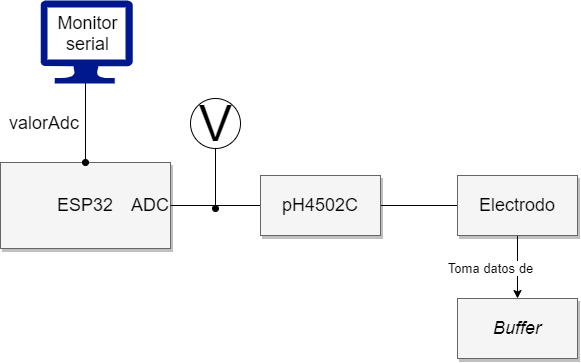
\includegraphics[width=0.7\textwidth]{./Figures/bancoPruebasCalibracion.png}
	\caption{Banco de pruebas para la calibración del electrodo.}
	\label{fig:bancoPruebasCalibracion}
\end{figure}

La tabla \ref{tab:ensayoCalibracion} muestra las mediciones correspondientes a cada unos de los valores de los \textit{buffers}, en un ambiente con temperatura de 25 °C. 

\begin{table}[h]
	\centering
	\caption[Resultados calibración.]{Datos obtenidos durante el proceso de calibración.}
	\begin{tabular}{c c c }    
		\toprule
		\textbf{\textit{Buffer} [pH]} & \textbf{Salida pH4602C [V] }	&    \textbf{Lectura ADC}  \\
		\midrule
		4 	& 2,635 & 3050 \\		
		7	& 2,172 & 2455 \\
		10	& 1,877 & 2120 \\
		\bottomrule
		\hline
	\end{tabular}
	\label{tab:ensayoCalibracion}
\end{table}

La diferencia de potencial entregada por el módulo pH4502C fue medida por un voltímetro y se representa en la segunda columna, mientras que el valor leído por el ADC se visualiza en la computadora a través de un monitor serial. Este valor es un número directamente proporcional a la tensión, con un valor de 0 para 0 V y un valor de 4095 para 3,5 V.

A partir de los datos obtenidos se puede graficar la recta de ajuste que relaciona el valor de pH con el valor medido por el ADC, como se muestra en la figura \ref{fig:rectaADC}. Los valores de pendiente y ordenada al origen calculados en el ESP32 fueron visualizados por el monitor serial. El valor m de la pendiente fue de -0,0063 y el valor de la ordenada al origen b fue de 22,98. 

\begin{figure}[htbp]
	\centering
	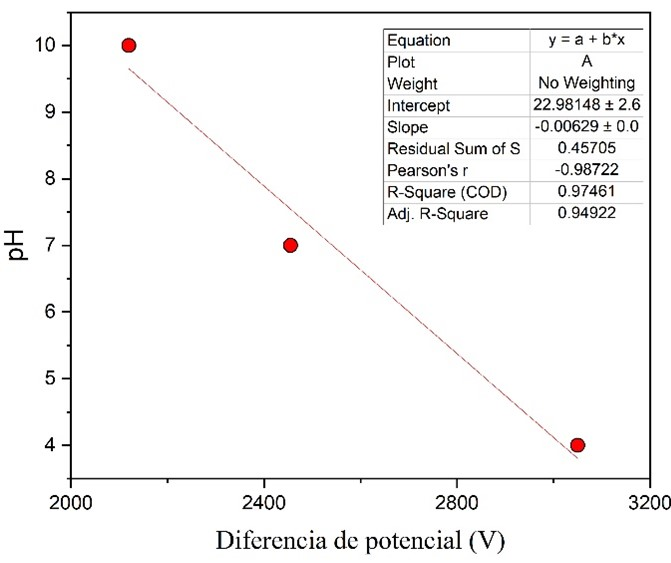
\includegraphics[width=0.7\textwidth]{./Figures/rectaADC.jpg}
	\caption{Relación entre el pH y el valor convertido por el ADC.}
	\label{fig:rectaADC}
\end{figure}

Luego de repetir el ensayo, se obtuvo que el error en la medición del potencial de salida del módulo pH4502C es de ± 1 mV, mientras que en la conversión a pH el error es de ± 0,1 pH a temperatura ambiente. 

\subsection{Calibración del volumen inyectado por la bomba}

El control de la bomba se realiza utilizando un esquema de lazo abierto, es decir que, cuando se inyecta líquido, el microcontrolador  no realiza una medición del caudal o del volumen que fue desplazado. A raíz de esto, surge la necesidad de establecer una relación entre la cantidad de micro pasos que realiza el motor y la cantidad de volumen que dosifica la bomba. Esto permite tener una unidad de medida y verificar si cumple con los requerimientos establecidos. Esta relación es difícil de obtener de manera teórica mediante el uso de modelos, por lo que se decidió realizar una serie de dosificaciones de un líquido de densidad conocida y pesar la cantidad dosificada para determinar el volumen.
El banco de pruebas utilizado para realizar este ensayo se muestra en la figura \ref{fig:bancoPruebasBomba}. En este proceso el fluido a dosificar fue agua de red domiciliaria, con una densidad estimada de 1 g/mL, y se utilizó una balanza de hasta 200 g con un error de ±0,01 g. El agua fue pesada en un vaso de precipitado previamente tarado.

\begin{figure}[htbp]
	\centering
	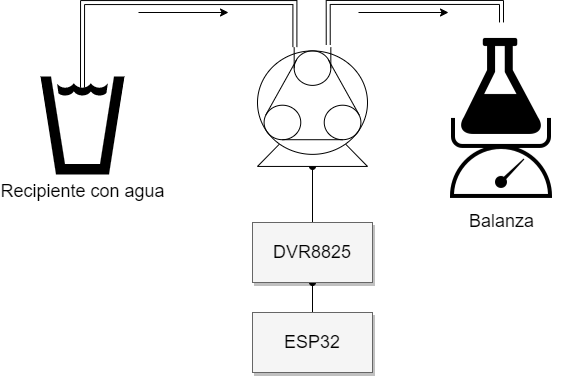
\includegraphics[width=0.7\textwidth]{./Figures/bancoPruebasBomba.png}
	\caption{Banco de pruebas para la calibración de la bomba.}
	\label{fig:bancoPruebasBomba}
\end{figure}

Se realizaron 10 dosificaciones, cada una de las cuales implicó un tiempo de 10 segundos y 100000 micro pasos para el motor, a una velocidad constante de 93,75 rpm. Se registró el peso y se taró nuevamente la balanza para todas las dosificaciones. Esta relación entre el número de pasos y el peso se muestra en la tabla \ref{tab:ensayoBomba}. La serie de mediciones arroja un peso medio de 0,87 g con un desvío de ± 0,01 g.

\begin{table}[h]
	\centering
	\caption[Dosificaciones]{Dosificaciones para el cálculo de volumen por paso.}
	\begin{tabular}{c c }    
		\toprule
		\textbf{Número de dosificación} & \textbf{Peso [g] } \\
		\midrule
		1 	& 0,87 \\	
		2	& 0,87 \\
		3	& 0,86 \\
		4	& 0,87 \\
		5	& 0,87 \\
		6	& 0,86 \\
		7	& 0,87 \\
		8	& 0,87 \\
		9	& 0,88 \\
		10	& 0,86 \\
		\bottomrule
		\hline
	\end{tabular}
	\label{tab:ensayoBomba}
\end{table}

La ecuación \ref{ec:pasosML} muestra el cálculo realizado para hallar la cantidad de micro pasos necesarios para dosificar 1 mL. Como resultado se tiene un valor de 114942 micro pasos por cada mL inyectado, lo que implica un tiempo de 11494,2 ms. Luego de realizar pruebas con este nuevo tiempo, se ajustó finalmente a 11500 ms para 1 mL y a 1150 ms para 0,1 mL.

\begin{equation}
\frac{Micro\:pasos\:realizados}{\frac{peso}{densidad}} = \frac{100000 [micro\:pasos]}{\frac{0,87 [g]}{1[\frac{g}{mL}]}}\:=\:114942 \:[\frac{micro\:pasos}{mL}]
\label{ec:pasosML}
\end{equation}

\vspace{1,5 cm}


\section{Validación y verificación}
\label{sec:validacionVerificacion}

Para la validación del prototipo se desarrolló un caso de uso completo en presencia de un analista químico. A continuación se detallan cada una de las actividades realizadas:
\begin{itemize}
	\item Calibración del electrodo con los 3 \textit{buffers}.
	\item Configuración del volumen de corte.
	\item Proceso de limpieza.
	\item Titulación de 50 mL de HCI 0,0500 M con NaOH 0,100 M.
	\item Visualización de resultados en la memoria micro SD y en la página web.
\end{itemize}

El banco de pruebas utilizado se muestra en la figura \ref{fig:bancoPruebasCompleto}

\begin{figure}[htbp]
	\centering
	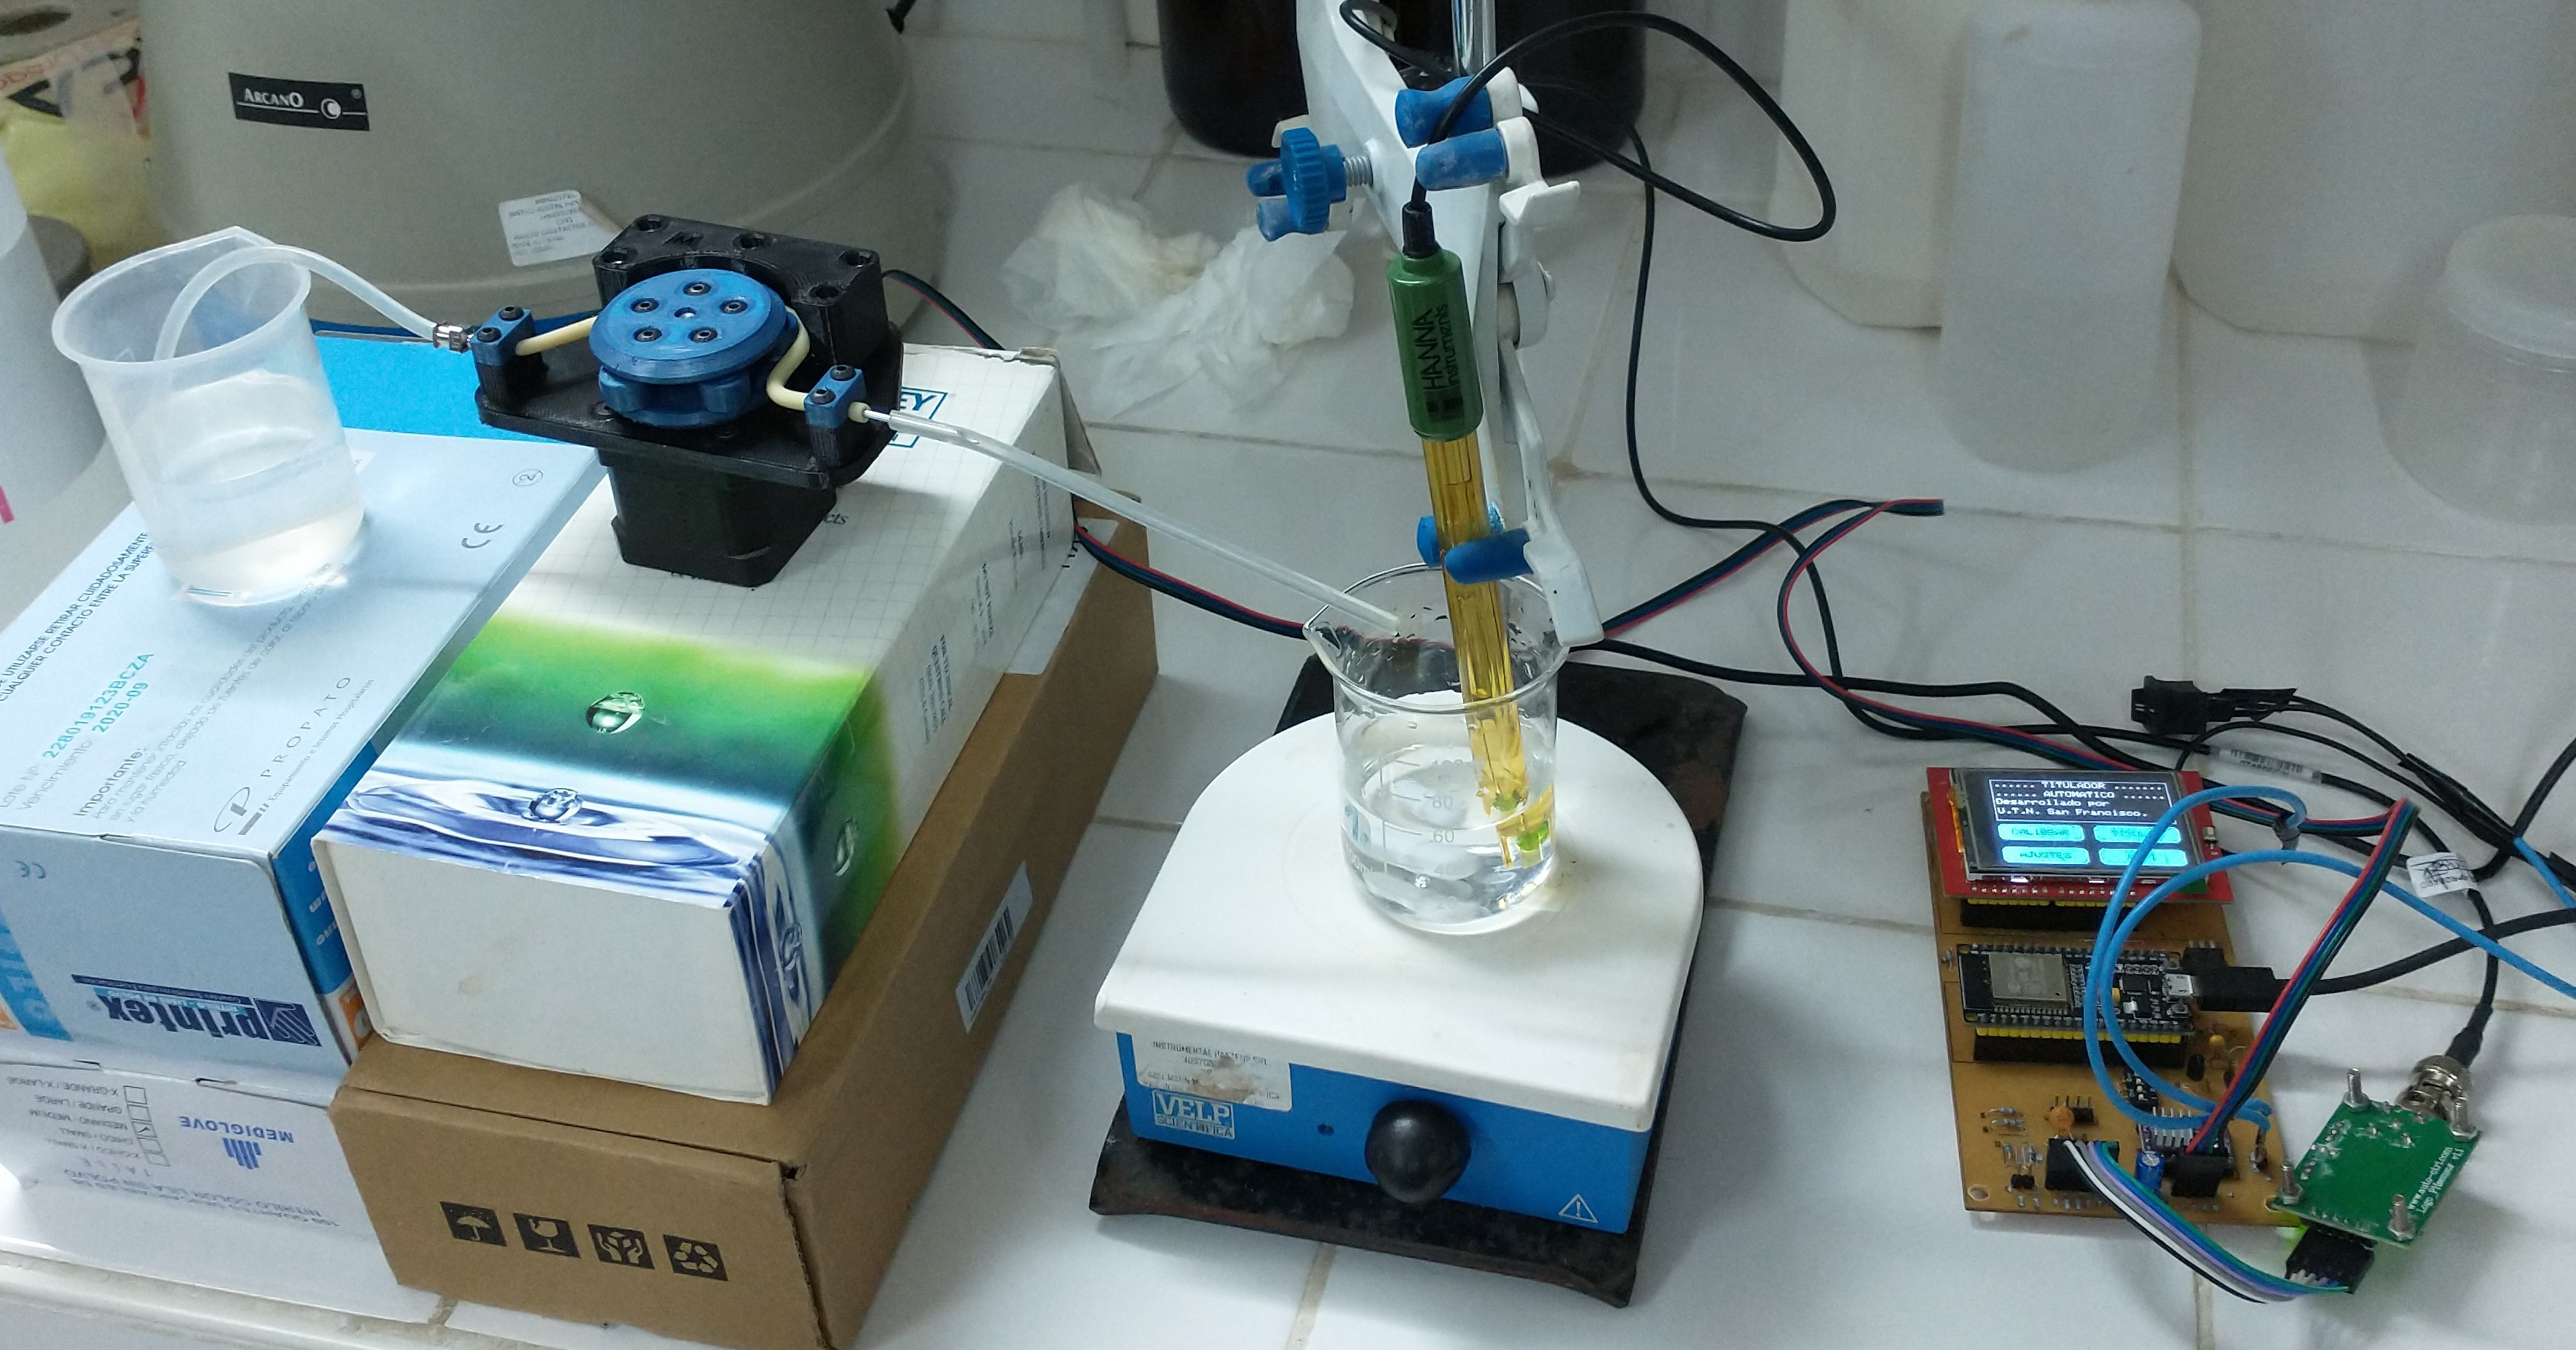
\includegraphics[width=0.9\textwidth]{./Figures/casoTitulacion.jpg}
	\caption{Banco de pruebas para el caso de uso.}
	\label{fig:bancoPruebasCompleto}
\end{figure}

La calibración del electrodo inicia cuando se ingresa en la opción CALIBRAR de la pantalla táctil. Allí se presiona la opción de BUFFER 4 y se coloca el \textit{buffer} correspondiente en un recipiente. Luego se introduce el electrodo y cuando la medición se estabiliza se presiona GUARDAR. Se realiza el mismo procedimiento para el resto de los \textit{buffers} y finalmente se presiona REGRESAR. En figura \ref{fig:casoParte1} se muestra la secuencia correspondiente a uno de los \textit{buffers}.

\begin{figure}[htbp]
	\centering
	\includegraphics[width=0.7\textwidth]{./Figures/casoParte1.png}
	\caption{Proceso de calibración.}
	\label{fig:casoParte1}
\end{figure}

Luego de la calibración y previo a la titulación es necesario realizar la limpieza con el titulante para eliminar las impurezas y purgar las mangueras de la bomba. Además, se debe establecer el valor del volumen de corte, que para este caso se fijó en 35 mL. En la figura \ref{fig:casoParte2} se muestran las pantallas correspondientes a estos procesos.

\begin{figure}[htbp]
	\centering
	\includegraphics[width=0.7\textwidth]{./Figures/casoParte2.png}
	\caption{Volumen de corte y limpieza.}
	\label{fig:casoParte2}
\end{figure}

A continuación se realiza la titulación. El tipo de titulación realizada es la que se muestra como ejemplo en el capítulo \ref{Chapter1}, sección \ref{subsec:curvas}. Una vez que el analista coloca el titulante y la muestra en los recipientes correspondientes, se da inicio a la tiluación mediante el botón TITULAR. El proceso comienza automáticamente y se visualiza la gráfica de pH respecto al tiempo. Luego de aproximadamente 10 minutos, el proceso finaliza y muestra en pantalla el volumen calculado en el punto final. Las pantallas correspondientes se muestran en la figura \ref{fig:casoParte3}.

\begin{figure}[htbp]
	\centering
	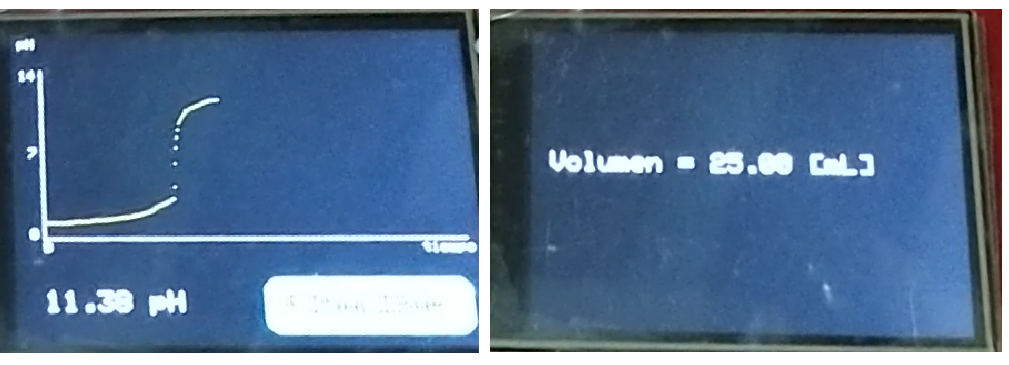
\includegraphics[width=0.7\textwidth]{./Figures/casoParte3.png}
	\caption{Curva de titulación y resultado.}
	\label{fig:casoParte3}
\end{figure}

En este instante se puede actualizar la página web y extraer el archivo de la memoria micro SD para visualizar el resultado y cada uno de los datos registrados, tal y como muestran las figuras \ref{fig:resultadoWeb.jpg} y \ref{fig:resultadoSD}, respectivamente. Se observa que el volumen en el punto final es de 25 mL, al igual que el modelo teórico visto anteriormente.

\begin{figure}[htbp]
	\centering
	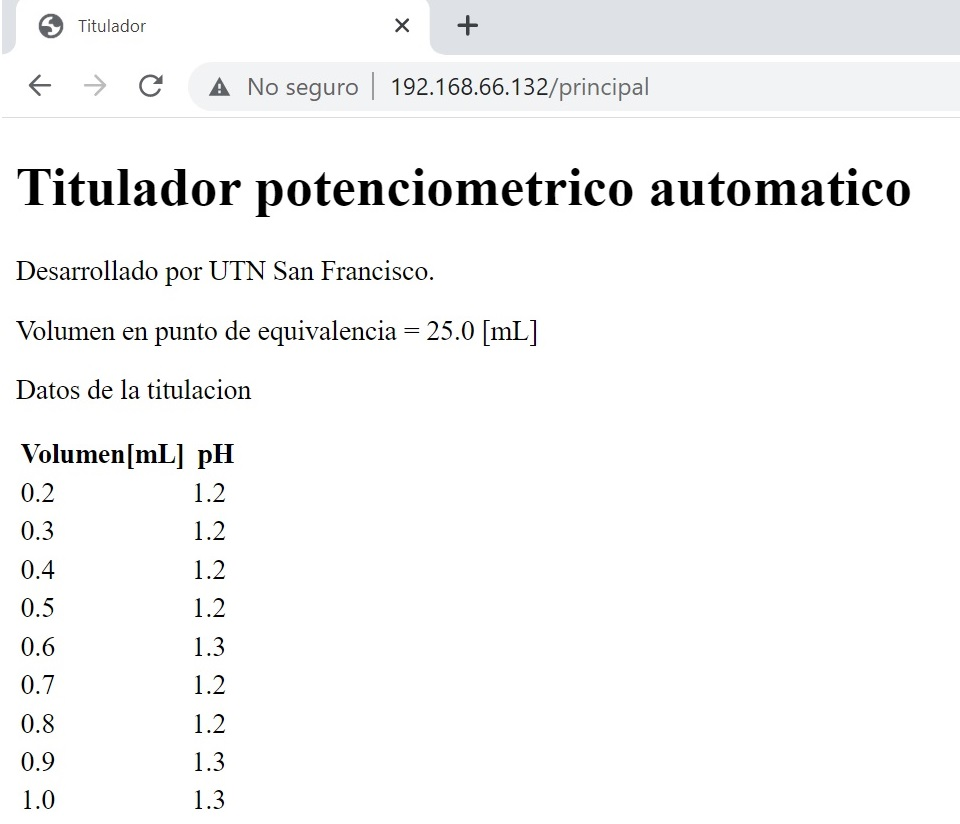
\includegraphics[width=0.742\textwidth]{./Figures/resultadoWeb.jpg}
	\caption{Resultado en página web.}
	\label{fig:resultadoWeb.jpg}
\end{figure}

\begin{figure}[htbp]
	\centering
	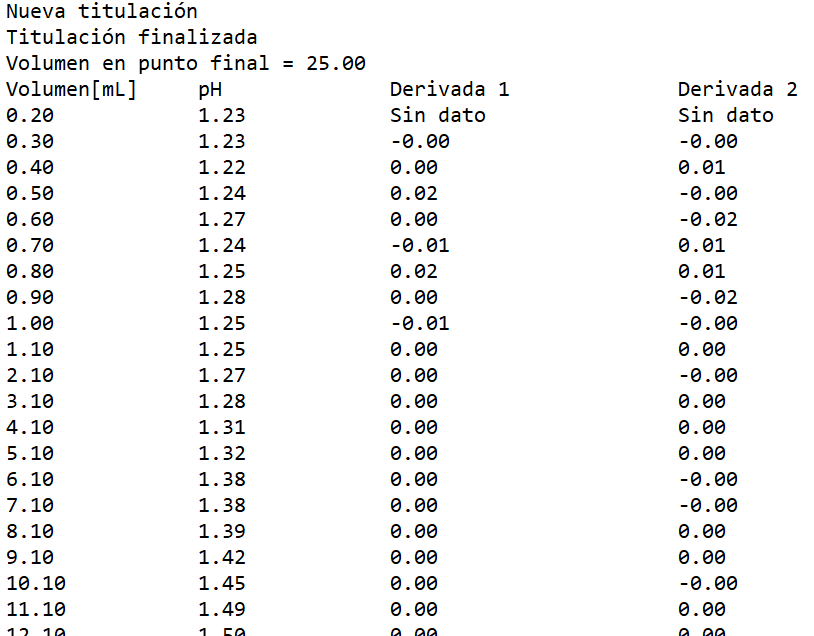
\includegraphics[width=0.742\textwidth]{./Figures/resultadoSD.png}
	\caption{Resultado en archivo de texto.}
	\label{fig:resultadoSD}
\end{figure}

\vspace{1,5 cm}

\section{Comparación con el estado del arte}

La tabla \ref{tab:titComparativa} muestra la comparativa entre el trabajo realizado y los tituladores automáticos analizados en la sección \ref{sec:estadoArte}. En la segunda columna se muestra la exactitud de dosificación en mL, para una bureta de 50 mL en los tituladores comerciales. Se observa que la exactitud lograda en este trabajo es la misma que la de uno de los tituladores comerciales analizados. En cuanto a la pantalla, esta es más pequeña que la de los comerciales y respecto las interfaces, si bien son diferentes, cumplen la función de llevar los datos a una computadora para su posterior procesamiento.

\begin{table}[h]
	\centering
	\caption[Comparativa con el trabajo realizado.]{Comparativa de tituladores comerciales con el trabajo realizado.}
	\begin{tabular}{l c c c }    
		\toprule
		\textbf{Marca y modelo} & \textbf{Exactitud [mL]}	&    \textbf{Display }&\textbf{Interfaces}  \\
		\midrule
		Kem AT710 		 	& 0,05 & 5,7" 		& RS232, USB \\		
		Mettler Toledo G20	& 0,10 & 5,7" Touch	& Ethernet, COM, USB \\
		Hanna HI901C1-01	 	& 0,05 & 5,7"		& VGA, USB, RS232 \\
		Trabajo realizado 	& 0,10 & 2,4" Touch	& micro SD, Wi-Fi \\
		\bottomrule
		\hline
	\end{tabular}
	\label{tab:titComparativa}
\end{table}